% LREC 2026 Example; 
% LREC Is now using templates similar to the ACL ones. 
\documentclass[10pt, a4paper]{article}

% This assumes your files are encoded as UTF8
\usepackage[utf8]{inputenc}

\usepackage{booktabs} % For formal tables
\usepackage{colortbl}
\usepackage{array}
\usepackage{multirow}
\usepackage{ragged2e}
\usepackage{hhline}
\usepackage{hyperref}


\usepackage[review]{lrec2026} % this is the new style
% the 'review' option anonymizes the paper following submission guideline
% the 'final' option produces the camera ready version (non anonymized)
% default version is 'final', so use review option for submission

\title{Efficient Adaptation of English Language Models for Low-Resource and Morphologically Rich Languages: The Case of Arabic}

\author{Ahmed Eldamaty \\
Giza Systems \\
Cairo, Egypt \\
\texttt{ahmed.aldamati@gizasystems.com} \\
\And Mohamed Maher \\
University of Tartu \\
Tartu, Estonia \\
\texttt{mohamed.abdelrahman@ut.ee} \\
\And Mohamed Mostafa \\
Giza Systems \\
Cairo, Egypt \\
\texttt{ibrahim.mohamed@gizasystems.com} \\
\And Mariam Ashraf \\
Giza Systems \\
Cairo, Egypt \\
\texttt{mariam.ashraf@gizasystems.com} \\
\And Radwa ElShawi \\
University of Tartu \\
Tartu, Estonia \\
\texttt{radwa.elshawi@ut.ee} \\}

\name{Ahmed Eldamaty, Mohamed Maher, Mohamed Mostafa, Radwa Elshawi} 

\address{Giza Systems, University of Tartu, Giza Systems, University of Tartu \\
         \{ahmed.aldamati, ibrahim.mohamed@gizasystems.com\}@gizasystems.com\\
         \{mohamed.abdelrahman, radwa.elshawi\}@ut.ee\\}


\abstract{
Transformer-based language models have revolutionized natural language processing, yet their adaptation to morphologically rich and underrepresented languages remains challenging. In this work, we introduce \texttt{ModernAraBERT}, a resource-efficient adaptation of the English-pretrained \texttt{ModernBERT} to Arabic. Our approach leverages continued pretraining on large curated Arabic corpora, followed by lightweight task-specific fine-tuning with frozen encoder backbones. This strategy preserves cross-lingual knowledge while effectively capturing Arabic morphology, offering a practical alternative to training monolingual models from scratch.  
We evaluate \texttt{ModernAraBERT} across three representative Arabic NLP tasks—sentiment analysis (SA), named entity recognition (NER), and extractive question answering (QA) using widely adopted benchmarks. Results show consistent improvements over the established \texttt{AraBERT v1} baseline and competitive performance relative to \texttt{mBERT}. Notably, \texttt{ModernAraBERT} yields gains of up to $\approx$17\% in SA, and significant improvements in NER and span-based QA metrics. Analysis further highlights trade-offs between accuracy and efficiency: while \texttt{ModernAraBERT} requires higher GPU memory than \texttt{AraBERT}, it provides superior downstream accuracy, especially for sentence and span level tasks.  
Beyond Arabic, our findings demonstrate that language-adaptive pretraining offers a scalable framework for extending state-of-the-art English models to other morphologically rich or low-resource languages, thereby reducing duplication of effort and broadening NLP inclusivity.
 \\ \newline \Keywords{Language Modeling, Less-Resourced, Named-Entity Recognition, Summarization, Sentiment Analysis} }

\begin{document}

%\begin{verbatim}
%\usepackage[review]{lrec2026}
%\end{verbatim}

\maketitleabstract
\section{Introduction}
Transformer encoder models such as BERT~\cite{devlin-etal-2019-bert} have revolutionized the approach to language processing tasks, especially within the English language. These models are characterized by their robustness, versatility, and success in numerous NLP applications and language representation tasks~\cite{Gardazi2025}. The Arabic language presents distinctive challenges: it is morphologically rich, replete with inflections, and encompasses various dialects. Consequently, adapting existing models trained in English to Arabic entails unique difficulties~\cite{MATRANE2023101570}.


Recent developments in Arabic NLP have been notably driven by the integration of deep learning and transformer-based architectures. The release of \texttt{AraBERT} as a pretrained model for Modern Standard Arabic (MSA) marked the inception of many subsequent Arabic BERT-based models~\cite{antoun2020arabert}. Some focus specifically on MSA, such as \texttt{CAMeLBERT}~\cite{inoue-etal-2021-interplay} and \texttt{ARBERT}~\cite{abdul-mageed-etal-2021-arbert}, which utilized carefully curated data. Others target dialectical variations, including \texttt{MARBERT}~\cite{abdul-mageed-etal-2021-arbert} and \texttt{QARiB}~\cite{abdelali2021pretraining}. Such models, though effective, often incur high computational costs and require training from scratch or extensive adaptation without efficient transfer or reduction in training duplication. Another widely used model is multilingual BERT (\texttt{mBERT})~\cite{devlin2018bert,alammary2022bert}. Unlike the Arabic-specific variants, \texttt{mBERT} was pretrained on Wikipedia data covering 104 languages, including Modern Standard Arabic. Its architecture consists of 12 transformer layers with 768 hidden units each, 12 self-attention heads, and approximately 110M trainable parameters.

Recently, significant advancements have been made through the introduction of \texttt{ModernBERT}~\cite{warner2024modernbert}, which modernizes encoder-only transformer architectures. \texttt{ModernBERT} addresses the critical limitations of previous models by training on an extensive dataset of 2 trillion tokens. Its architecture integrates several efficiency and performance improvements, such as rotary positional embeddings (RoPE)~\cite{su2024roformer}, alternating global-local attention layers, and the utilization of GeGLU activation functions~\cite{shazeer2020glu}. These architectural enhancements, combined with a modern tokenizer optimized for diverse textual and code-related data, enable \texttt{ModernBERT} to achieve state-of-the-art performance in a broad spectrum of classification and retrieval tasks, thus providing an optimal foundation for adapting advanced language models to languages with unique linguistic challenges, such as Arabic.


The main contributions of this paper can be summarized as follows.
\begin{itemize}
\item We propose a resource-efficient strategy to extend high-performing English language models to Arabic by conducting efficient pretraining on curated Arabic corpora, thus providing a practical alternative by adapting an existing English-pretrained model to Arabic, instead of developing an entirely new Arabic-specific model from scratch.

\item We present \texttt{ModernAraBERT}, an adapted version of the state-of-the-art English \texttt{ModernBERT} model, specifically fine-tuned and optimized for Arabic NLP tasks.

\item We empirically evaluate \texttt{ModernAraBERT} across three essential Arabic NLP benchmarks: sentiment analysis, named entity recognition, and question answering, demonstrating its superior performance compared to \texttt{AraBERT v1} and \texttt{mBERT} baselines. Our approach significantly reduces computational overhead, enhancing accessibility and applicability for research communities and industry practitioners working with Arabic language processing.

\item We empirically evaluate \texttt{ModernAraBERT} across three essential Arabic NLP benchmarks: sentiment analysis, named entity recognition, and question answering against two strong baselines: \texttt{AraBERT v1}, the most widely recognized and cited Arabic BERT model with performance comparable to later variants~\cite{antoun2020arabert,farha2021benchmarking}, and \texttt{mBERT}, a widely adopted multilingual model covering Arabic among 104 languages~\cite{alammary2022bert}. Our results show that \texttt{ModernAraBERT} consistently outperforms both models while reducing computational overhead.

\end{itemize}



\section{Methodology}

Our methodology builds on that large-scale English-pretrained models encode transferable cross-lingual knowledge that can be effectively adapted to morphologically rich languages such as Arabic. Instead of training a new Arabic-specific model from scratch, which is both computationally costly and resource intensive, we employ continued pretraining on curated Arabic corpora. This strategy preserves the syntactic and semantic priors acquired during large-scale English pretraining, while adapting the model to capture Arabic-specific morphology and orthographic variations. Prior studies have demonstrated that domain and language-adaptive pretraining often yields superior performance compared to monolingual training under resource constraints~\cite{gururangan-etal-2020-dont,pfeiffer-etal-2021-adapterfusion}. Moreover, multilingual models such as \texttt{mBERT} have shown that English initialization can rival or even surpass dedicated Arabic models (e.g., \texttt{AraBERT}) in certain tasks~\cite{alammary2022bert}. Our approach thus provides a scalable and resource-efficient alternative to monolingual pretraining, while ensuring comparability with established baselines.


\subsection{Pretraining Corpora}
We compiled a large-scale Arabic corpus from four publicly available sources: OSIAN~\cite{zeroual-etal-2019-osian}, the Arabic Billion Words dataset~\cite{el20161}, the Arabic Wikipedia dump\footnote{\href{https://dumps.wikimedia.org/arwiki/}{https://dumps.wikimedia.org/arwiki/}}, and the OSCAR Arabic dataset~\cite{2022arXiv220106642A}. These corpora jointly cover Modern Standard Arabic (MSA) and a variety of dialectal forms.  

Preprocessing included:  
\begin{itemize}
    \item Diacritics removal: to reduce sparsity arising from inconsistent annotation across sources.  
    \item Elongation (tatweel) removal: to eliminate stylistic markers that do not contribute semantic value.  
    \item Punctuation and special characters removal: to reduce noise from web and social media text.  
\end{itemize}  

To enhance morphological representation, we applied the Farasa segmenter~\cite{abdelali2016farasa} for affix and root segmentation. The final corpus contained over six million sentences, totaling approximately 17~GB of normalized Arabic text.

\subsection{Tokenization}

We extended the original \texttt{ModernBERT} tokenizer, which was trained on English corpora, by adding 80,000 Arabic-specific tokens. The extended vocabulary included segmented roots, inflected forms, and common affixes, ensuring that Arabic morphology was more faithfully captured. Frequent morphological constructions were explicitly added as standalone tokens to improve segmentation consistency and reduce fragmentation.  

The choice of 80K tokens was empirically validated. As shown in Figure~\ref{fig:vocab}, Arabic follows a long-tailed frequency distribution, where most tokens occur rarely. Our analysis of token frequency (left) and coverage versus vocabulary size (right) demonstrates that coverage improves sharply with vocabulary size but plateaus around 80K tokens. Beyond this point, additional tokens provide negligible coverage gains. Selecting 80K therefore balances corpus coverage with computational efficiency. This cutoff is also consistent with prior Arabic BERT models: \texttt{AraBERT} employs a 64K vocabulary, while \texttt{MARBERT} uses 95K.  

\begin{figure*}[h]
\centering
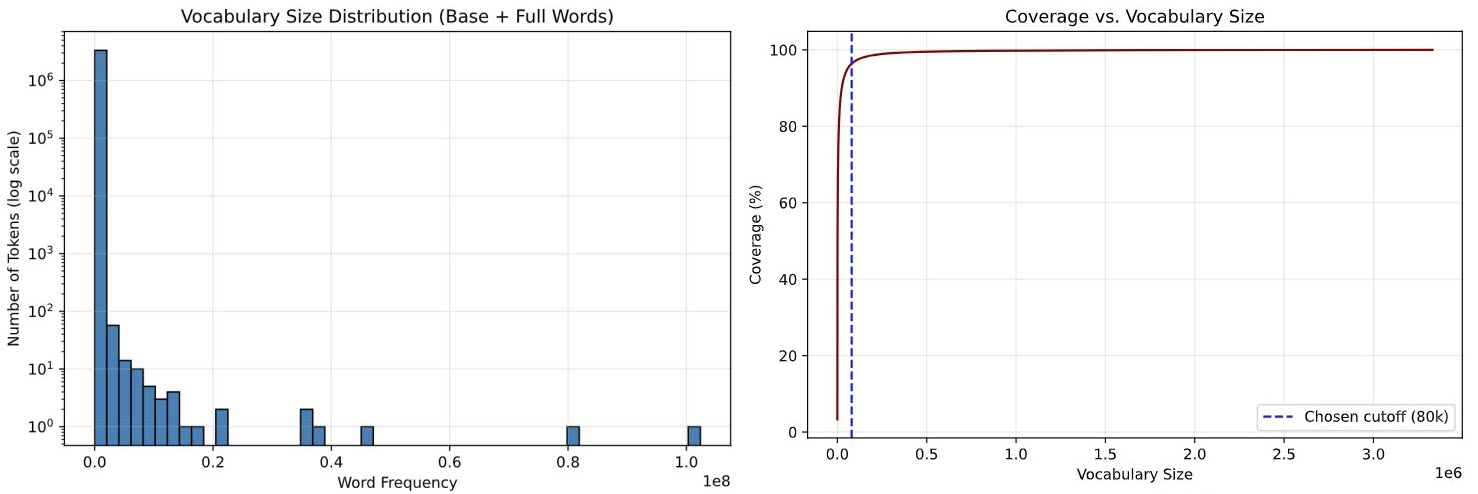
\includegraphics[width=\linewidth]{80k.jpg}
\caption{Vocabulary size analysis. Left: Token frequency histogram (log scale). Right: Coverage vs. vocabulary size, with the chosen cutoff at 80K tokens.}
\label{fig:vocab}
\end{figure*}

\subsection{Model Training}
Our model is based on the publicly available \texttt{ModernBERT}-base\footnote{\href{https://huggingface.co/answerdotai/ModernBERT-base}{ModernBERT-Base}} architecture with 22 transformer layers (Figure~\ref{fig:model}). To accommodate the extended vocabulary, we resized the embedding layer accordingly.  

Pretraining was conducted with the Masked Language Modeling (MLM) objective, updating all model parameters. Training proceeded for three epochs: the first two epochs used sequences of length 128 for efficiency, while the final epoch employed sequences of 512 to model longer contexts. The context length was restricted to 512 tokens both to ensure fair comparability with \texttt{AraBERT} (which also uses 512) and to fit within the 40~GB GPU memory available. Longer contexts (e.g., 8,192 tokens) were not computationally feasible under our hardware constraints. 
Optimization used AdamW with cosine learning rate decay and gradient clipping. Training progress was monitored via loss and perplexity on a held-out validation set.  

\begin{figure}[!ht]
\begin{center}
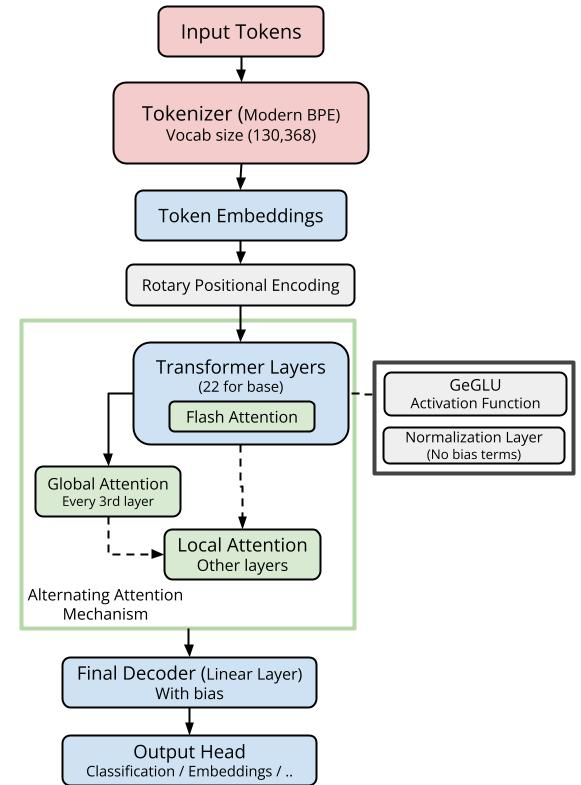
\includegraphics[width=\columnwidth]{LREC2026 Author's kit/ModernArabert (1).jpg}
\caption{ModernBERT architecture with extended tokenizer vocabulary size and embedding layer.}
\label{fig:model}
\end{center}
\end{figure}

The pretrained \texttt{ModernAraBERT} will be released on HuggingFace\footnote{\href{http://}{URL to be revealed after double-blind review}}, together with training and evaluation scripts in our repository\footnote{\href{https://anonymous.4open.science/r/ModernAraBERT-823C/}{Repository link}}.
%https://huggingface.co/gizadatateam/ModernAraBERT
%https://github.com/giza-data-team/ModernAraBERT

\section{Experimental Setup}

To assess the effectiveness of our proposed adaptation strategy, we evaluate \texttt{ModernAraBERT} on three representative Arabic NLP tasks: sentiment analysis (SA), named entity recognition (NER), and extractive question answering (QA). These tasks were chosen as they collectively cover sentence-level, sequence-labeling, and span-extraction settings, providing a comprehensive evaluation of model capabilities. We compare against two strong baselines: \texttt{AraBERT v1}, the most established Arabic-specific BERT variant, and \texttt{mBERT}, a widely adopted multilingual model.  

All experiments follow a controlled fine-tuning protocol where the pretrained encoder is kept frozen, and only lightweight task-specific heads are optimized. This setup isolates the contribution of continued pretraining on Arabic corpora, while reducing the risk of overfitting on limited task data. Detailed descriptions of hardware, datasets, and training configurations are provided below.

\subsection{Computational Environment}
All pretraining and fine-tuning experiments were conducted on a high-performance computing node equipped with 12 CPU cores, 32~GB RAM, and a 40~GB NVIDIA A100 GPU. These specifications constrained the choice of sequence length (512 tokens) to ensure comparability with \texttt{AraBERT} while remaining feasible within GPU memory.  

\subsection{Fine-Tuning Strategy}
During this phase, the pretrained encoder parameters were frozen and only the task-specific classification heads were fine-tuned. This strategy was selected to 
(i) reduce training time,  
(ii) minimize overfitting on relatively small task datasets, and  
(iii) assess the quality of representations obtained during continued pretraining.  

Unless otherwise specified, all tasks were trained with a maximum of 200 epochs, early stopping patience of 10 epochs, AdamW optimizer, and a dropout ratio of 0.1 for regularization. An exception was NER, which converged reliably within 5 epochs.

\subsection{Sentiment Analysis}
We benchmarked sentiment classification using three datasets:  
\begin{itemize}
    \item \textbf{Hotel Arabic Reviews Dataset (HARD)}~\cite{Elnagar2018}, comprising reviews in both Modern Standard Arabic (MSA) and dialectal Arabic. Following~\cite{antoun2020arabert}, we excluded neutral 3-star reviews, yielding a binary classification setting.  
    \item \textbf{Arabic Jordanian General Tweets (AJGT)} Corpus\footnote{\href{https://github.com/komari6/Arabic-twitter-corpus-AJGT}{AJGT Dataset}}, containing 1,800 tweets labeled as positive or negative.  
    \item \textbf{Large-Scale Arabic Book Reviews (LABR)}~\cite{aly-atiya-2013-labr}, using the unbalanced binary version for consistency with prior work.  
\end{itemize}  

For datasets without predefined splits, we followed a 60/20/20 train/validation/test partition. Sentence-level representations were derived from the \texttt{[CLS]} token and passed to a classification head for binary or multi-class prediction. Performance was measured using Macro F1-score.  

\subsection{Named Entity Recognition}
NER experiments were performed on the ANERCorp dataset~\cite{Benajiba:2007}, using the official CAMeL Lab splits provided via HuggingFace~\cite{obeid2020camel}. The dataset includes entities such as \texttt{Person}, \texttt{Location}, and \texttt{Organization}.  

We adopted the IOB2 tagging scheme~\cite{Ramshaw1999}. To ensure correct alignment under subword tokenization:  
- the first subtoken of each word was assigned the gold entity label,  
- continuation subtokens were either mapped to the corresponding I-label (e.g., \texttt{B-PER} $\rightarrow$ \texttt{I-PER}) if available, or masked with \texttt{-100} during loss computation.  

This setup ensures entity-level consistency and avoids label fragmentation across subtokens. A token classification head was placed above the encoder, with evaluation reported as micro F1-score at the entity level, following established NER practice.  

\subsection{Question Answering}
For extractive QA, we combined Arabic-SQuAD~\cite{Mozannar:2019} with 50\% of ARCD~\cite{mozannar-etal-2019-neural} as training data, reserving the remaining 50\% of ARCD for testing. This setup provides both coverage and comparability with prior Arabic QA studies.  

The QA head comprised the pretrained encoder, a prediction layer, and a linear classifier producing start and end span logits. Regularization was applied via dropout (0.1). Hyperparameters included 200 training epochs, AdamW optimizer (learning rate $3\times10^{-5}$), batch sizes of 64 for \texttt{AraBERT} and 32 for \texttt{ModernAraBERT}, and early stopping based on validation F1.  

Question–context pairs were tokenized to a maximum of 512 tokens with a document stride of 128 for long contexts. Character-level answer spans were mapped to token indices, and cross-entropy loss was computed jointly over start and end positions. During inference, the predicted answer span was extracted by selecting the start–end token pair with maximum joint probability.  

Evaluation followed standard extractive QA metrics: Exact Match (EM), token-level F1, and Sentence Match (SM), providing complementary measures of exactness, token overlap, and semantic alignment.  


In summary, our experimental setup was designed to provide a rigorous and fair evaluation of \texttt{ModernAraBERT}. We assessed the model across three complementary task types—sentence-level classification (SA), sequence labeling (NER), and span extraction (QA)—using widely adopted benchmark datasets. Comparisons against both Arabic-specific (\texttt{AraBERT v1}) and multilingual (\texttt{mBERT}) baselines ensure that our evaluation is representative of the state of the art. By freezing the encoder and fine-tuning only lightweight task-specific heads, we isolate the contribution of continued pretraining on Arabic corpora while controlling for overfitting. The following section presents the results of these experiments, highlighting both performance gains and computational trade-offs relative to the baselines.



\section{Results and Discussion}

This section reports the empirical results of \texttt{ModernAraBERT} on the three mentioned downstream Arabic NLP tasks. Our discussion emphasizes both absolute performance gains and relative improvements over baselines, highlighting the effectiveness of continued pretraining as well as any trade-offs observed.

\subsection{Sentiment Analysis}
Table~\ref{tab:sentiment_results} summarizes performance on the three sentiment datasets. Across all benchmarks, \texttt{ModernAraBERT} achieves substantial improvements over both \texttt{AraBERT v1} and \texttt{mBERT}, despite only fine-tuning the prediction head. This demonstrates that continued pretraining on Arabic corpora effectively enhances the model’s sentence-level representations, yielding strong transfer to downstream classification tasks.

Performance gains are particularly notable on the HARD dataset (+16.7~\% over \texttt{AraBERT}, +17.7~\% over \texttt{mBERT}), which contains both MSA and dialectal Arabic, indicating that the model captures cross-variant sentiment signals more effectively. On AJGT and LABR, improvements of 12.5~\% and 11~\% respectively confirm robustness across both small-scale (tweets) and large-scale (book reviews) corpora. These consistent gains suggest that \texttt{ModernAraBERT} generalizes well across domains and genre variations.

\begin{table}[ht]
    \centering
    \label{tab:sentiment_results}
    \begin{tabular}{l@{\hspace{0.25cm}}c@{\hspace{0.25cm}}c@{\hspace{0.25cm}}c}
        \toprule 
        \textbf{Dataset} & \textbf{AraBERT} & \textbf{mBERT} & \textbf{ModernAraBERT} \\
        \midrule 
        AJGT  & 58.0  & 61.5 & \textbf{70.5} \\
        HARD  & 72.7 & 71.7 & \textbf{89.4} \\
        LABR  & 45.5 & 45.5 & \textbf{56.5} \\
        \bottomrule
    \end{tabular}\\
    \caption{Macro-F1 (\%) on sentiment datasets.}
    \vspace{0.1cm}
\end{table}







\subsection{Named Entity Recognition (NER)}
\label{sec:ner_results}
Table~\ref{tab:ner_results} reports the NER results on ANERCorp. \texttt{ModernAraBERT} achieved a micro F1-score of 82.1~\%, surpassing \texttt{AraBERT v1} (78.9\%) while remaining below \texttt{mBERT} (90.7\%). These results highlight two important observations. First, continued pretraining on Arabic corpora improves token-level representation quality relative to \texttt{AraBERT}, confirming the benefits of our adaptation strategy for sequence labeling. Second, the superior performance of \texttt{mBERT} indicates that multilingual training at scale may provide broader cross-lingual generalization for this task, potentially due to larger training diversity and multilingual alignment.  

%We also examined computational efficiency. \texttt{AraBERT} achieved higher throughput (925.4 samples/sec vs. 495.8 for \texttt{ModernAraBERT}) and required less VRAM (0.52~GB vs. 0.83~GB), while RAM usage was comparable (1.30~GB vs. 1.41~GB). This points to a trade-off: \texttt{ModernAraBERT} offers higher accuracy than \texttt{AraBERT}, but at the cost of slower inference and higher GPU memory consumption.  

\begin{table}[ht]
    \centering
    \label{tab:ner_results}
    \begin{tabular}{l@{\hspace{0.3cm}}c}
        \toprule \textbf{Model} & \textbf{Micro F1} \\
        \midrule 
        AraBERT~\cite{antoun2020arabert} & 78.9 \\
        mBERT                           & \textbf{90.7} \\
        ModernAraBERT                   & 82.1 \\
        \bottomrule
    \end{tabular}\\
    \caption{Named Entity Recognition results (Micro F1-score, \%) on \texttt{ANERCorp}.}
    \vspace{0.1cm}
\end{table}

\subsection{Question Answering (QA)}
Results for the QA task are presented in Table~\ref{tab:qa_results}. \texttt{ModernAraBERT} consistently outperformed both baselines across all evaluation metrics. Compared to \texttt{AraBERT}, our model achieved a 41.3\% relative gain in Exact Match (18.73 vs. 13.26), a 15.6\% relative gain in F1-score (47.18 vs. 40.82), and a 7.3\% relative gain in Sentence Match (76.66 vs. 71.47). These improvements indicate that \texttt{ModernAraBERT} not only produces more exact matches but also captures semantic information more effectively at both token and sentence levels.  

Interestingly, while \texttt{mBERT} performed competitively (15.27 EM, 46.12 F1-Score), it lagged behind in Sentence Match (63.11), suggesting weaker ability to capture longer-span semantic coherence. By contrast, \texttt{ModernAraBERT} demonstrated stronger semantic alignment, which we attribute to the continued pretraining on Arabic corpora and task-specific fine-tuning.  

\begin{table}[ht]
    \centering
    \small
    \label{tab:qa_results}
    \begin{tabular}{l@{\hspace{0.25cm}}c@{\hspace{0.25cm}}c@{\hspace{0.25cm}}c}
        \toprule \textbf{Model} & \textbf{EM} & \textbf{F1} & \textbf{SM} \\
        \midrule 
        AraBERT~\cite{antoun2020arabert} & 13.26 & 40.82 & 71.47 \\
        mBERT                           & 15.27 & 46.12 & 63.11 \\
        ModernAraBERT                   & \textbf{18.73} & \textbf{47.18} & \textbf{76.66} \\
        \bottomrule
    \end{tabular}\\
    \caption{Extractive QA results (\%) on \texttt{ARCD} Test Split.}
    \vspace{0.1cm}
    \footnotesize \textit{EM: Exact Match, F1: token-level F1, SM: Sentence Match.}
\end{table}


\subsection{Overall Analysis}
Across all evaluated tasks, adapting an English pretrained model to Arabic through our two phase strategy continued pretraining followed by task-specific fine-tuning proved highly effective. \texttt{ModernAraBERT} consistently outperformed the Arabic-specific \texttt{AraBERT v1} 
% TODO: add NER and mBERT if we outperformed it
baseline, with particularly strong gains in sentiment analysis and question answering. These improvements confirm that resource-efficient language adaptation can rival or surpass monolingual models trained from scratch.  

At the same time, results underscore important trade-offs. While \texttt{ModernAraBERT} achieved higher accuracy, \texttt{AraBERT} maintained superior inference throughput achieving a higher throughput of 925.4 samples/sec vs. 495.8 for \texttt{ModernAraBERT} and lower GPU memory usage, especially evident in NER experiments. This suggests that model selection should be guided by application requirements: latency-critical or resource-constrained scenarios may favor \texttt{AraBERT}, whereas accuracy-oriented deployments benefit more from \texttt{ModernAraBERT}. The competitive performance of \texttt{mBERT} in NER further highlights the potential of large multilingual pretraining for token-level tasks, though it lagged behind in sentence-level semantic alignment (SM) for QA.  

\subsection{Hardware Resource Usage}
Table~\ref{tab:hardware_usage} summarizes peak memory consumption across benchmarks. A consistent pattern emerges: \texttt{AraBERT} is the most memory-efficient model, while \texttt{ModernAraBERT} incurs higher VRAM usage, particularly for QA (3.22~GB vs.~2.07~GB for \texttt{AraBERT}). RAM usage remained broadly similar across models, with only minor fluctuations.  

These findings confirm that \texttt{ModernAraBERT} offers accuracy improvements at the cost of increased GPU memory demand, especially in span-extraction tasks. From a practical perspective, this trade-off is acceptable for research and enterprise environments with sufficient GPU capacity, but may limit deployment on edge devices or latency-sensitive pipelines. By contrast, \texttt{AraBERT} remains attractive for lightweight applications, while \texttt{mBERT} provides a balanced middle ground for scenarios requiring cross-lingual portability.  

\begin{table}[!ht]
\label{tab:hardware_usage}
\begin{center}
\small
\begin{tabularx}{\columnwidth}{|l|l|X|X|}
      \hline
      \textbf{Benchmark} & \textbf{Model} & \textbf{Peak RAM} & \textbf{Peak VRAM} \\
      \midrule 
      \multirow{3}{*}{NER} & AraBERT & 1.53 & 0.52 \\
                           & mBERT & 1.60 & 0.68 \\
                           & ModernAraBERT & 1.49 & 0.83 \\
      \hline
      \multirow{3}{*}{QA}  & AraBERT & 1.42 & 2.07 \\
                           & mBERT & 1.46 & 2.84 \\
                           & ModernAraBERT & 1.39 & 3.22 \\
      \hline
      \multirow{3}{*}{SA}  & AraBERT & 1.65 & 0.52 \\
                           & mBERT & 1.66 & 0.68 \\
                           & ModernAraBERT & 1.36 & 0.82 \\
      \hline
\end{tabularx}
\caption{Hardware resource usage across models and benchmarks (GB).}
\end{center}
\end{table}

Although our experiments focus on Arabic, the proposed methodology is inherently language-agnostic. By leveraging English-pretrained backbones such as \texttt{ModernBERT} and applying language-adaptive pretraining on target corpora, similar strategies can be employed for other morphologically rich or low-resource languages. This reduces the need to train monolingual models from scratch, a process that is often prohibitively expensive in both data and compute.  
The results suggest that languages with limited dedicated resources may benefit disproportionately from this approach. For instance, languages such as Amharic, Urdu, or Kazakh—which face challenges of sparse annotated data and high morphological complexity could be supported through continued pretraining on monolingual corpora while reusing the cross-lingual knowledge encoded in large English models~\cite{Wiemerslage2022MorphologicalPO}.  

From a community perspective, this paradigm promotes inclusivity by lowering the barrier to building competitive NLP models for underrepresented languages. It complements multilingual models like \texttt{mBERT} by offering a targeted, resource-efficient alternative that can achieve stronger task-specific performance without requiring massive multilingual pretraining. Thus, the broader impact of our work lies in presenting a scalable framework for extending state-of-the-art NLP to languages that remain marginalized in the current landscape of large language models.


\section{Conclusion}

This paper introduced \texttt{ModernAraBERT}, a resource-efficient adaptation of the English-pretrained \texttt{ModernBERT} model to Arabic. Our approach leverages continued pretraining on curated Arabic corpora followed by lightweight task-specific fine-tuning. Experimental results across three representative tasks—sentiment analysis, named entity recognition, and question answering—demonstrated that \texttt{ModernAraBERT} consistently outperforms the widely used \texttt{AraBERT v1} baseline and achieves competitive results against the multilingual \texttt{mBERT}.  The results highlight important trade-offs. While \texttt{ModernAraBERT} improves accuracy, especially in sentence- and span-level tasks, it incurs higher GPU memory usage and slower inference compared to \texttt{AraBERT}. This suggests that model selection should be deployment-specific: lightweight models for latency-critical scenarios, and adapted models like \texttt{ModernAraBERT} for accuracy-oriented applications.  

Beyond Arabic, our approach has a broader applicability of language-adaptive pretraining as a scalable alternative to monolingual model development. The methodology can be extended to other morphologically rich or underrepresented languages, offering a pathway to reduce duplication of effort while maintaining strong downstream performance.  

In future work, we plan to (i) explore mixed adaptation strategies combining language and domain adaptive pretraining, (ii) investigate parameter-efficient tuning techniques to further reduce memory overhead. We believe these directions will strengthen the case for resource-efficient cross-lingual adaptation as a practical paradigm for building inclusive NLP systems.



%\section{Acknowledgements}

%Place all acknowledgments (including those concerning research grants and funding) in a separate section at the end of the paper.


\nocite{*}
\section{Bibliographical References}
%\section{References}
\label{sec:reference}
\bibliographystyle{lrec2026-natbib}
\bibliography{lrec2026-example}

\section{Language Resource References}
\label{lr:ref}
\bibliographystylelanguageresource{lrec2026-natbib}
\bibliographylanguageresource{languageresource}


\end{document}
